\section{A calibrated confounding alarm with a predictable power frontier}
\label{sec:detection}

The detection problem is $H_0\colon \gamma=0$ against $H_1\colon \gamma=g\,\mathrm{dir}$ with $g=\|\gamma\|$ and $\|\mathrm{dir}\|=1$, observed through the standardized pair $(\tilde Y,X_c)$, where $\tilde Y$ is $Y$ centered and rescaled to unit sample variance. Throughout, $c=p/n$, $\hat w=X_c^{\top}\tilde Y/n$ is the sample cross-moment, and $(d_j,v_j)$, $j=1,\dots,p$, are the eigenpairs of the sample covariance $\hat\Sigma=X_c^\top X_c/n$. The alarm we ship is deliberately selective: it listens only to the coordinates through which supercritical confounding ($l_j>\sqrt c$) must express itself \citep{bbp2005phase,benaychgeorges2012singular}, and it pays for that selectivity with a price we characterize exactly.

\subsection{Construction}

For each selected coordinate $j\le k$, where $k$ comes from an Onatski-type eigenvalue-ratio edge selector \citep{onatski2010determining} applied to $\hat\Sigma$ and capped at ten coordinates, define
\[
z_j=\frac{\sqrt n\, v_j^\top \hat w}{\sqrt{d_j}},
\qquad
T_{\max}=\max_{j\le k}\frac{|z_j|}{\sqrt{\widehat{\mathrm{var}}_j}},
\qquad
\widehat{\mathrm{var}}_j=\frac{\hat\sigma_\varepsilon^2+d_j/c}{\hat\sigma_y^{\,2}},
\]
with the two nuisance estimates following one shared frozen convention: both the residual-variance estimate $\hat\sigma_\varepsilon^2$ and the response-scale estimate $\hat\sigma_y^2$ are computed on the same standardized pair from the trimmed residual variance after spike removal, so that no estimator sees data the other did not.\footnote{$\hat\sigma_\varepsilon^2$ is the bulk-median estimator: the median of sub-edge sample eigenvalues divided by the Marchenko--Pastur median at aspect $\min(c,1)$, capped at the observed bulk median; $\hat\sigma_y^{\,2}=\mathrm{mean}(d)+\hat\sigma_\varepsilon^2$, the observable form of $\mathrm{tr}(\hat\Sigma)/p+\sigma_\varepsilon^2$ under A4a. The same two estimates drive the tuning path, so alarm calibration and estimator tuning cannot drift apart.} The statistic $T_{\max}$ (S2, \emph{maxz\_cal}) rejects above a threshold, and two threshold conventions are carried side by side: the frozen gate rule reads $T_{\max}$ against the matched-null Monte Carlo 95th percentile, while the arithmetic fallback applies the two-sided Gaussian Bonferroni cut $z_{1-0.05/(2k)}$. The variance law inside the calibration is exact rather than heuristic: conditional on the design, $\mathrm{Var}(z_j)=(\sigma_\varepsilon^2+d_j/c)/\sigma_y^2$ under $H_0$, because the Haar draw of the regression vector leaks into every rowspace coordinate with variance $d_j/c$, a leakage tax that grows exactly where $p\gg n$.

\subsection{Why the finite-\texorpdfstring{$n$}{n} null is not Gaussian-max, and why that became a derivation target}

The naive mental model treats the $z_j$ as independent standard Gaussians and reads $T_{\max}$ against a Bonferroni quantile. The measured matched-null 95th percentile of the calibrated statistic runs at roughly $1.7$ times that naive scale, a gap large enough to demand explanation rather than patching, and the explanation became a derivation target in its own right. First, a conditional independence lemma: under $H_0$ the pairwise covariances of the calibrated coordinates vanish identically, eigenvector orthogonality killing both the loading channel and the noise channel, so the correct null model is a maximum over independent coordinates with unequal scales, not correlated chi-squares. Second, the inflation is a marginal-scale effect: the realized null law $\kappa_{n,k}$ of $T_{\max}$ factorizes into a dominant scale-calibration ratio, produced by the nuisance estimator pair (validated against $c\le 1$ bulk geometry, it systematically mis-scales on the $n$-side spectrum when $c>1$; at $c=5$ the scale credited at the top coordinate misses by about $20\%$, with measured $4.21$ against a credited $3.50$), times an exact max-over-$k$ term that stays within $(0.9,1.05]$ for $k\le 10$, plus a documented positive spread correction from per-replicate fluctuation of the nuisance estimates, a Jensen effect for ratios. The assembled statement, carried at deterministic-equivalent level in Supplementary Document S-B, is the following.

\begin{lemma}[Conditional independence of calibrated coordinates under $H_0$]
\label{lem:condindep}
Under $H_0$ and conditionally on the sample eigenpairs $(d_j,v_j)$, the standardized coordinates satisfy
$\mathrm{Cov}(z_j,z_{j'})\mid (d,v)=0$ for $j\ne j'$, with $\mathrm{Var}(z_j)=(\sigma_\varepsilon^2+d_j/c)/\sigma_y^2$.
At deterministic-equivalent level the coordinates are therefore independent Gaussians with these variances.
\end{lemma}

\begin{proof}[Proof]
Write $z_j=\sqrt n\,v_j^\top \hat w/\sqrt{d_j}$ with $\hat w=X_c^\top\tilde Y/n$; under $H_0$ the standardized response keeps its signal piece, $\tilde Y=(X_c\beta+\varepsilon)/\sigma_y$, which is what produces the leakage term below. Conditional on $(d,v)$, $\tilde Y$ is Gaussian, so each $z_j$ is Gaussian with the exact conditional variance $\mathrm{Var}(z_j)=(\sigma_\varepsilon^2+d_j/c)/\sigma_y^2$ displayed in the Construction above: the $d_j$ piece is the signal-coordinate projection of $\tilde Y$ through the design and the $d_j/c$ piece is the leakage tax of the Haar draw of the regression vector. For $j\ne j'$, eigenvector orthogonality $v_j^\top v_{j'}=0$ kills both the shared loading channel and the shared noise channel of the covariance exactly, so the joint Gaussian law factorizes.
\end{proof}

\begin{remark}[Empirical null-law decomposition]
\label{prop:nullfactor}
Grant Lemma~\ref{lem:condindep}. Then, at deterministic-equivalent level with discrepancy terms $o_p(1)$ after standardization, the calibrated statistic admits the decomposition
\[
T_{\max}\;=\;c_n\cdot M_k\cdot(1+\Delta_n)+o_p(1),
\]
where every factor is measurable from matched-null output alone: $M_k=\max_{j\le k}|N_j|$ is the maximum of $k$ independent standard normals, whose standardized quantiles lie within $[0.9,1.05]\cdot z_{1-0.05/(2k)}$ for $k\le10$; $c_n\ge0$ is the ratio of realized coordinate scales to their nominal conditional values; and $\Delta_n\ge0$, recovered as the residual ratio once $c_n$ and $M_k$ are removed, collects the Jensen-type effect of replicate fluctuation in the nuisance estimates. This statement records the decomposition and the measurability of its factors from matched-null output; its convergent content (rates for $c_n$ and $\Delta_n$) is carried in Supplementary Document S-B, so the proposition should be read as an empirically closed decomposition rather than a limit theorem.
\end{remark}

The measured matched-null 95th percentile sits at about $1.7\times$ the naive Gaussian-maximum scale. The dominant contributor is scale miscalibration on the $n$-side spectrum when $c>1$, quantified at roughly $20\%$ on the top coordinate at $c=5$ (measured $4.21$ against credited $3.50$) and larger on inner coordinates where the leakage term $d_j/c$ enters; the remainder is carried by $\Delta_n$. This is why the shipped threshold is the matched-null Monte Carlo quantile rather than an analytic cut.

The calibration evidence is at scale. Across the $31$ audited null cells of the null-calibration sweep, which totals $39{,}200$ matched replicate pairs including its supporting alignment and twin configurations, the noise-aware evaluation against true size $0.05$ returns pooled $\chi^2$ $p=0.4114$, maximum standardized deviation $2.91$, and $96.8\%$ of cells within $\pm 2$ standard deviations: statistically indistinguishable from perfect calibration. We co-report the less flattering arithmetic. The raw share of cells landing inside the frozen band $[0.035,0.065]$ is $80.65\%$, a number that mostly measures replication budgets, since at $500$ to $1200$ replicates per cell the split-half standard error reaches $0.014$, comparable to the band's entire half-width. The raw Bonferroni convention shows median size $0.1625$, quantifying the same $1.7\times$ looseness from the other side. Finally, the scree baseline S0 records median analytic ``size'' $1.0$ under $\gamma=0$, by construction and by design: scree detects the population spikes themselves rather than confounding \citep{johnstone2001distribution}, so naive visibility alarms fire on every spiked design, confounded or not.

\subsection{The power frontier}

The predictor assembles the same objects the null law identified: per-coordinate mean shifts placed at the BBP sample locations with capture-weighted couplings, the $d_j/c$ leakage tax, and the matched-null percentile as threshold scale. One approximation is declared up front. The frozen predictor treats the calibrated shift as linear in $g$, whereas the true shift scales like $g/\sqrt{A+g^2}$ with $A=1+\sigma_\varepsilon^2$, because response self-normalization deflates couplings as the confounding strengthens; inside the gated strength range this bends slopes by under $15\%$, well inside the pre-declared factor-$1.5$ tolerance.

The predeclared acceptance band for frontier agreement is a factor of $1.5$ in either direction on the strength axis; every ratio below is read against it. Evaluation is gated to the three strata whose direction carries supercritical-aligned mass: mixed profile, $\theta=\pi/6$, $c\in\{0.2,0.8,2.0\}$, $n=2000$. Empirical $g$ at $80\%$ power lands inside the band in every case, with ratios of empirical to predicted $0.93$, $1.25$, and $1.02$ across increasing $c$; the median ratio is $1.02$ and the share of gated strata within factor $1.5$ is exactly $1.0$. The worst cell ($c=0.8$, mixed profile, $\theta=\pi/6$) predicts $g_{\mathrm{pred}}=0.261$ against empirical $g_{80}=0.325$, a ratio of $1.246$, still comfortably passing. Figure~\ref{fig:power} overlays the full power surfaces on the predicted frontiers.

\begin{figure}[t]
\centering
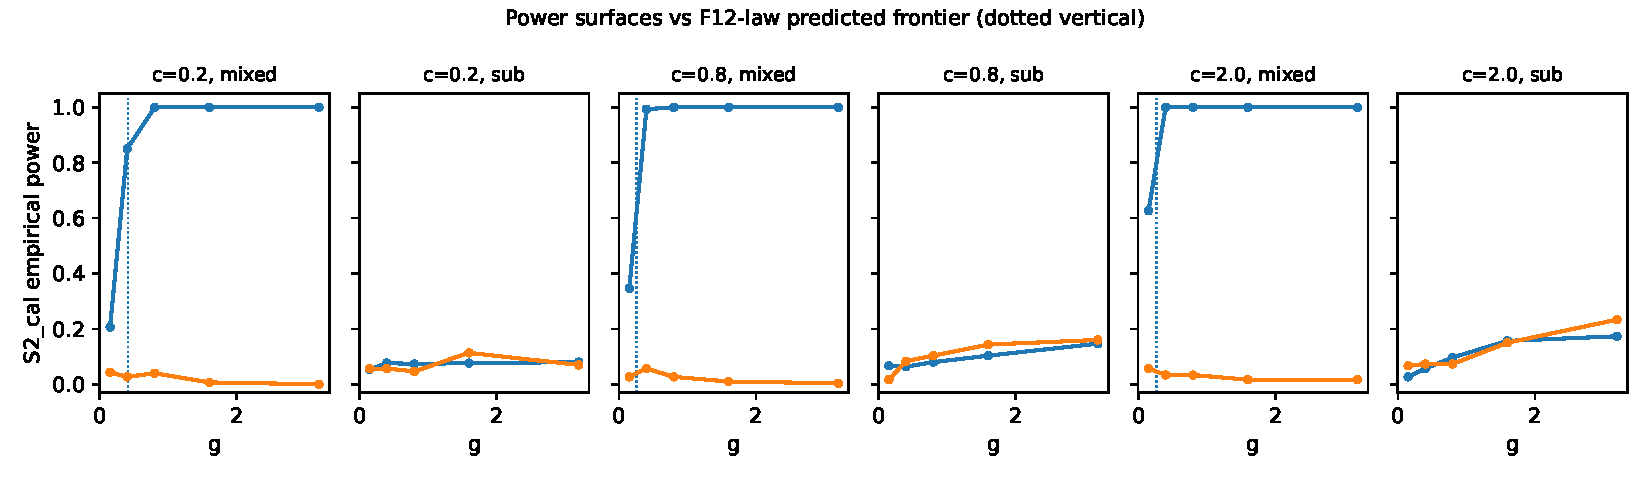
\includegraphics[width=\textwidth]{figures/power_surface_vs_frontier.pdf}
\caption{Empirical power of the calibrated alarm S2 against confounding strength $g$ for the simulation strata ($n=2000$), overlaid on the frozen frontier predictions built from the exact null-variance law with capture-weighted BBP locations and the $d_j/c$ leakage tax. Supercritical-aligned strata (mixed profile, $\theta=\pi/6$) track the predicted $80\%$ contour within a factor of about one (ratios $0.93$, $1.25$, $1.02$; median $1.02$). Strata without supercritical-aligned mass remain at or below $0.25$ power at the largest simulated strength $g=3.2$.}
\label{fig:power}
\end{figure}

In the nine remaining strata the prediction is an infinite frontier: fully subcritical spike profiles, or mass concentrated on the subcritical second factor near $\theta=\pi/2$. All nine strata confirm the forecast, with empirical power at or below $0.25$ at the largest simulated strength $g=3.2$ (confirmed in $9$ of $9$ strata). This is not a finite-sample accident but a ceiling.

\begin{proposition}[Subcritical power ceiling]
\label{prop:ceiling}
Fix a subcritical profile ($l_j<\sqrt c$ for all $j$) and any fixed $g$. The overlap of every sample eigenvector with the coherent confounding direction is $O_p(n^{-1/2})$ \citep{benaychgeorges2012singular}, so the calibrated coordinate means stay tight and the asymptotic power of $T_{\max}$ at level $\alpha$ converges to
\[
\mathrm{pow}_\infty(g)=\Pr\Big(\max_j\big|\mu_j^{\mathrm{tight}}(g)+\kappa_j N_j\big|>\mathrm{thr}\Big)\;<\;1,
\]
a constant strictly below one, where $\kappa_j$ are the realized null scales and $\mathrm{thr}$ the calibrated threshold.
\end{proposition}

\begin{proof}[Proof sketch]
Under $H_0$ the calibrated coordinates are asymptotically independent with tight scales $\kappa_j$ (the conditional-independence lemma established above), and subcriticality makes every coherent mean shift tight as well: each coordinate mean is $O_p(n^{-1/2})$ because sample eigenvector overlaps with the fixed confounding direction collapse at rate $n^{-1/2}$ \citep{benaychgeorges2012singular}. Hence $\mathrm{pow}_\infty(g)=\Pr(\max_{j\le k}|\mu_j+\kappa_j N_j|>\mathrm{thr})$, a maximum over finitely many independent continuous variables with bounded shifts; since each coordinate places positive probability below $\mathrm{thr}$, the complement is nonempty and the supremum is strictly below one.
\end{proof}

Measured maxima in the blind strata, $0.17$ to $0.25$ at $g=3.2$ and rising only slowly in $g$, match a saturating mean-shift law rather than a slow escape. ``Infinite frontier'' is thus gate shorthand for a precise statement: no accessible strength reaches $80\%$ power, and the honest asymptotic bound sits strictly below one. What the alarm cannot see, by which mechanisms, and exactly where quadratic summaries go blind as well, is the business of Section~\ref{sec:blindness}.
